% Paper A, IEEE conference format (MoSICom 2026: IEEE template, typically 6 pages). The body and every number come from
% docs/paper/latex/main.tex (the measured draft of 2026-10-05); see docs/paper/PRE_SUBMISSION_NOTES.md.
\documentclass[conference]{IEEEtran}
\renewcommand{\ttdefault}{cmtt}   % Courier is not installed locally
\usepackage{cite}
\usepackage{amsmath}
\usepackage{booktabs}
\usepackage{graphicx}
\usepackage{tikz}
\usetikzlibrary{positioning,arrows.meta,fit}
\usepackage{url}
\usepackage[hidelinks]{hyperref}

\begin{document}

\title{Testing Text-to-SQL Warning Signals: A Pre-registered Study of Data Checks, Judges and Self-Consistency}

\author{\IEEEauthorblockN{Neel Pradeep Jaiswal, Ronak Daniel Ramanathan, Elizabeth Jish Joy and Hima Deepthi Vankayalapati}
\IEEEauthorblockA{Mukesh Patel School of Technology, Management and Engineering, NMIMS, Mumbai, India\\
neelpjaiswal@gmail.com, danielronak8105@gmail.com, jish.joy@nmims.edu, himadeepthi.vankayalapati@nmims.edu}}

\maketitle

\begin{abstract}
A text-to-SQL system should warn when an answer may be wrong, and many warning signals exist: data
checks with no model call, process signals, LLM judges, self-consistency. Comparing them fairly is
harder than it looks. In a pre-registered study on 393 held-out BIRD Mini-Dev questions we show three
choices that change the conclusions. Rarely-firing yes/no checks look useless under AUROC, so we
compare every signal with a judge at the same flag rate. Labels matter: corrected gold annotations
move accuracy by 10.7 points, and counting the remaining format-only errors as correct removes
self-consistency's lead over the judge. Cost matters: at one extra call each, the judge ranks answers
better than self-consistency (significantly for one of two models), which needs three samples to
draw level. Applied to data checks (row-multiplying
joins, truncated results, all-NULL aggregates, ungrounded figures), the result is negative: they apply
to 4\% of answers and catch no more errors than the judge at the same rate (9 vs.\ 10.8; 95\% CI of
the difference $-6.3$ to $2.2$), and a second SQL model gives the same picture. A blind annotation of
every error explains why: most errors are semantic. An agent retry is the best free warning (79\%
precision).
\end{abstract}

\begin{IEEEkeywords}
text-to-SQL, answer verification, selective prediction, LLM judges, self-consistency, pre-registration
\end{IEEEkeywords}

\section{Introduction}

Natural-language interfaces to databases are now good enough to deploy and still wrong often enough
to mislead. A business user who asks how many patients had an abnormal test and receives a confident
number cannot tell whether the query counted patients or lab tests. An honest ``this might be wrong''
attached to such answers is worth more than a slightly higher accuracy.

Two families of signals can provide it. \emph{Model-based} signals ask a model again: resample the
query and measure agreement (self-consistency), or ask a separate LLM to judge the answer; recent work
places black-box signals around 0.61--0.68 AUROC and LLM judges at 0.72--0.78~\cite{richardson2026predicts}. \emph{Data checks} inspect the answer against the database with no
model call. They are free, instant and explainable (``this join repeats each patient 46 times''),
which makes them attractive in a product.

We built such checks into a self-hosted text-to-SQL system and asked, in a pre-registered study,
whether they earn their place. Answering fairly took care that comparisons of such signals usually
skip, and that care changes the conclusions. Our contributions:
\begin{enumerate}
\item An evaluation protocol for correctness warnings: a matched-flag-rate primary measure that is fair
to rarely-firing yes/no checks, scoring against corrected annotations~\cite{jin2026annotation},
cost-matched comparison of sampling-based signals, and pre-registered hypotheses with Holm correction.
\item Evidence on BIRD Mini-Dev~\cite{li2023bird} that these choices matter: correction moves accuracy
by 10.7 points; a fifth of the remaining errors are format-only, and counting them as correct removes
self-consistency's lead over the judge; at equal cost the judge leads.
\item A negative result with its reason: data checks rarely apply (4--6\% of answers for two models) and
do not beat a judge; a blind annotation of every wrong answer (two annotators, $\kappa=0.74$; repeated
for the second model) shows most errors are semantic, and structural double-counting checks miss
double counting through legitimate joins.
\item Resources: a frozen fan-out set (60 risky, 33 control questions) on which current models
rarely double count (0 and 5 of 60), the annotations, and all run records, available on request.
\end{enumerate}

\section{Related Work}

\textbf{Correctness prediction.} Richardson~\cite{richardson2026predicts} compares black-box, white-box and
verification signals on BIRD and Spider; Somov and Tutubalina~\cite{somov2025confidence} study entropy-based selective
classifiers; Chen et al.~\cite{chen2025abstention} add abstention via conformal prediction on hidden states. All
of these signals come from a model. \textbf{Database feedback.} SQLens~\cite{gong2025sqlens} is the
closest work: it combines database signals (abnormal results, empty predicates, join-tree issues) with
LLM signals in a learned classifier. We instead evaluate data checks as warnings in their own right,
at a matched flag rate, on corrected labels, with pre-registered hypotheses and an error annotation
that explains what the checks can and cannot see. \textbf{Benchmark quality.}
Wretblad et al.~\cite{wretblad2024noise} document noise in BIRD; Jin et al.~\cite{jin2026annotation} report annotation errors
in 52.8\% of Mini-Dev and release corrections, which we score against. Execution match has false
negatives~\cite{pourreza2023evaluating,kim2025flex}; we quantify them after correction.
\textbf{Self-consistency}~\cite{wang2023selfconsistency} is applied here as agreement between the
execution results of resampled queries.

\section{System and Signals}

The system routes each question; for database questions an LLM writes SQL, a read-only gate validates
it, and it runs with a row cap. The model retries with a classified error message when a query fails
or returns nothing; a second call writes the answer from the first rows of the result. SQL and answers
are written by GPT-5 mini at its provider's default sampling (it accepts no temperature), reached through a third-party hosted-model service; Qwen3.8-27B (temperature 0) normalises
the question. The served model is recorded on every call. Fig.~\ref{fig:pipeline} shows the pipeline
and where each signal is read. A held-out question costs 9.0 model calls on average, of which 5 are
self-consistency samples.

\begin{figure}[t]
\centering
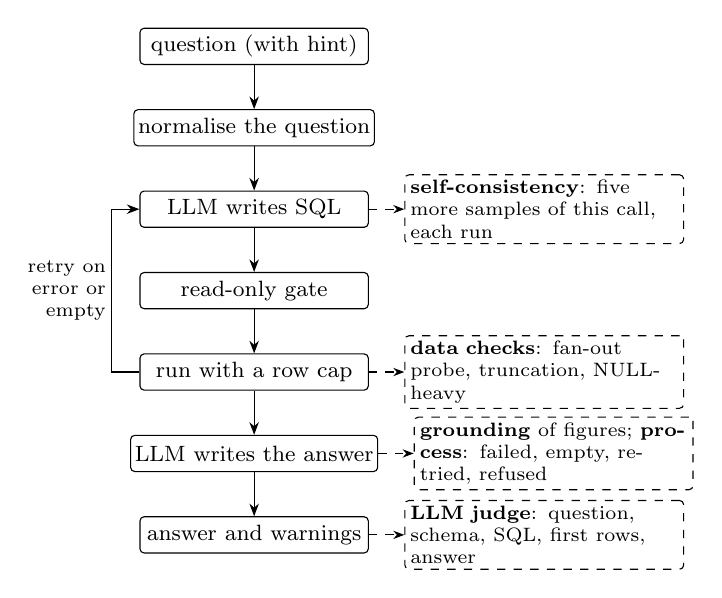
\begin{tikzpicture}[font=\footnotesize, node distance=5.6mm,
  stp/.style={draw, rounded corners=1.5pt, minimum width=29mm, minimum height=4.6mm, inner sep=1.5pt},
  sig/.style={draw, dashed, rounded corners=1.5pt, text width=34mm, align=left, inner sep=2pt, font=\scriptsize},
  flow/.style={-{Stealth[length=1.6mm]}}, tap/.style={dashed, -{Stealth[length=1.4mm]}}]
\node[stp] (q) {question (with hint)};
\node[stp, below=of q] (norm) {normalise the question};
\node[stp, below=of norm] (sql) {LLM writes SQL};
\node[stp, below=of sql] (gate) {read-only gate};
\node[stp, below=of gate] (run) {run with a row cap};
\node[stp, below=of run] (ans) {LLM writes the answer};
\node[stp, below=of ans] (out) {answer and warnings};
\draw[flow] (q)--(norm); \draw[flow] (norm)--(sql); \draw[flow] (sql)--(gate);
\draw[flow] (gate)--(run); \draw[flow] (run)--(ans); \draw[flow] (ans)--(out);
\draw[flow] (run.west) -- ++(-3.5mm,0) |- (sql.west);
\node[font=\scriptsize, align=right, left=4.2mm of gate, inner sep=0pt] {retry on\\error or\\empty};
\node[sig, right=4.5mm of sql]  (sc) {\textbf{self-consistency}: five more samples of this call, each run};
\node[sig, right=4.5mm of run]  (dc) {\textbf{data checks}: fan-out probe, truncation, NULL-heavy};
\node[sig, right=4.5mm of ans]  (pr) {\textbf{grounding} of figures; \textbf{process}: failed, empty, retried, refused};
\node[sig, right=4.5mm of out]  (jd) {\textbf{LLM judge}: question, schema, SQL, first rows, answer};
\draw[tap] (sql)--(sc); \draw[tap] (run)--(dc); \draw[tap] (ans)--(pr); \draw[tap] (out)--(jd);
\end{tikzpicture}
\caption{The pipeline (left) and where each warning signal is read (right). Data checks and process
signals need no model call.}
\label{fig:pipeline}
\end{figure}

\textbf{Data checks} (no model call): a \emph{fan-out probe} compares \texttt{COUNT(key)} with
\texttt{COUNT(DISTINCT key)} per joined table for aggregates over joins; \emph{truncation} (the result
hit the row cap); \emph{NULL-heavy} (an all-NULL aggregate); \emph{figure grounding} (every number in
the answer must trace to a result cell, a column aggregate, the question, or the number of rows shown
to the answer writer); and \emph{any data check}, their union. \textbf{Process baselines}: the query
failed, the result was empty, the agent needed a retry, the answer refuses. \textbf{Model baselines}:
an LLM judge (Gemini 3.8 Flash through the same service, primary; gpt-oss-120b, secondary; their mean as
an ensemble), each
from a different family than the SQL model and shown the question, schema, SQL, first rows and answer;
it is asked whether the result correctly answers the question and returns a probability with a
one-sentence reason. Self-consistency draws five more samples of the SQL call and runs each; its risk
is the share whose result differs from the answer's. The fan-out probe is the only check that explains
itself in the data's terms (``this join repeats each patient 46 times''); the others report a state of
the result.

\section{Study Design}

\textbf{Pre-registration.} The protocol was written before measuring. A 100-question pilot exposed
harness faults (a prompt rule that turned \texttt{LIMIT 1} into \texttt{LIMIT 1000}; grounding false
alarms from the pipeline's own wording; noisy original labels), and the protocol was revised before
any held-out question was asked. Pilot questions are development data, excluded from all results;
every amendment is logged with whether the pilot informed it.

\textbf{Data.} Mini-Dev has 498 unique questions; the 398 outside the pilot, minus 5 whose SQLite and
PostgreSQL copies disagree on the original gold, form the held-out set of 393. Labels are the
corrected annotations~\cite{jin2026annotation}, written for SQLite: gold runs on BIRD's SQLite
databases, predictions on the PostgreSQL copy, compared to five significant digits (validated on the
original golds of both copies: 491 of 498 agree). The \textbf{fan-out set} has 60 risky questions,
whose natural SQL aggregates a parent-level quantity across a one-to-many join, and 33 controls on the
same tables; each has a gold query, an independently written check query that must agree with it, and
the naive join, which must differ from gold (risky) or equal it (control). It was drafted with an LLM
from rules fixed in advance and frozen after one author reviewed a random 20\%.

\textbf{Measures.} The SQL label is execution match (relaxed: column order and extra columns ignored;
BIRD's strict rule also reported). The \emph{primary measure} is wrong answers caught at a matched
flag rate: when a signal flags $k$ answers, we compare its wrong answers with the expected number among
the judge's $k$ most suspect. Let $W$ be the wrong answers and $F_s$ the $k$ answers that signal $s$
flags. Order the answers by decreasing judge risk into tie groups $G_1, G_2, \dots$, and let $j$ be the
first group that does not fit entirely within the top $k$. Then
\begin{equation}
E_J(k)=\sum_{i<j}|G_i\cap W| \;+\; \frac{k-\sum_{i<j}|G_i|}{|G_j|}\,|G_j\cap W|,
\end{equation}
\begin{equation}
\Delta_s = |F_s\cap W| - E_J(k),
\end{equation}
so ties are broken at random in expectation, exactly, with no sampling. A yes/no check that fires on
4\% of answers has an AUROC near 0.5 whatever its precision; $\Delta_s$ asks instead whether its few
flags are better spent than the judge's. We also report precision, recall, AUROC and the area under the
risk--coverage curve (AURC: the mean error rate of the answers kept as the most suspect are withheld
one by one). For cost matching, self-consistency's risk is recomputed from $m$ of its five samples and
its AUROC averaged over all $\binom{5}{m}$ choices of samples. Statistics use a paired bootstrap
stratified by database (2,000 resamples) and Holm correction over four confirmatory tests: \textbf{H1}
the fan-out check beats the judge at its flag rate on the fan-out set; \textbf{H2} ordering by any
data check, then judge risk, lowers the judge's AURC; \textbf{H3} grounding flags fewer than 5\% of
correct answers; \textbf{H4} one evidence-guided repair fixes more than it breaks and adds 2 points.
H1 and H4 require at least 10 double-counting errors or repairs, else they are untestable; if the main
model fails H1's precondition, the set is rerun with a second model (gpt-oss-120b). Every wrong answer
was annotated blind to the signals into ten types; a second annotator (another model, on a reshuffled
blank copy) labelled all 90 ($\kappa=0.74$; 0.87 for system error vs.\ benchmark artefact).

\section{Results}

\textbf{Accuracy.} 77.1\% under the relaxed rule (95\% CI 72.5--81.2; strict 70.2\%); against the
original gold, 66.4\%. Counting the 20 errors whose only fault is output format as correct gives
82.2\% (exploratory).

\begin{table}[t]
\centering\small
\setlength{\tabcolsep}{3.5pt}
\begin{tabular}{lrrrr}
\toprule
signal & $k$ & prec. & rec. & vs.\ judge at $k$ (95\% CI) \\
\midrule
any data check & 17 & .53 & .10 & $-1.8$ ($-6.3$, $2.2$) \\
\quad fan-out & 1 & 1.00 & .01 & $+0.4$ \\
\quad truncation & 9 & .22 & .02 & $-3.7$ ($-7.4$, $-0.7$) \\
\quad NULL-heavy & 2 & 1.00 & .02 & $+0.7$ \\
\quad grounding & 5 & .80 & .04 & $+0.8$ ($-1.2$, $2.8$) \\
query failed & 4 & 1.00 & .04 & $+1.5$ ($0.4$, $2.9$) \\
empty result & 6 & 1.00 & .07 & $+2.2$ ($0.7$, $4.1$) \\
needed a retry & 24 & .79 & .21 & $+3.7$ ($-1.7$, $8.6$) \\
refusal & 7 & .57 & .04 & $-0.5$ ($-2.7$, $1.7$) \\
\bottomrule
\end{tabular}
\caption{Warnings on the held-out set (90 of 393 wrong). Last column: wrong answers the signal catches
minus the judge's expected catch among its $k$ most suspect answers. Failed and empty queries are wrong
by construction here: no corrected gold result is empty.}
\label{tab:signals}
\end{table}

\begin{figure}[t]
\centering
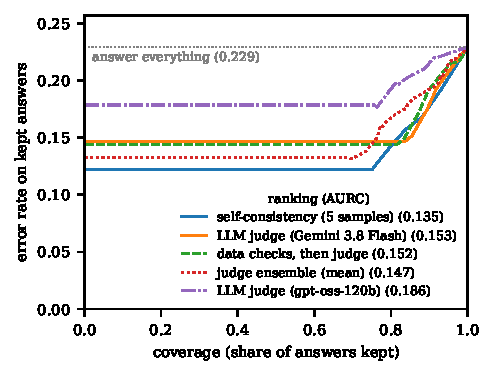
\includegraphics[width=\columnwidth]{../fig_risk_coverage.pdf}
\caption{Risk--coverage on the held-out set. Flat segments are large ties: most answers get the
lowest risk from every ranking.}
\label{fig:rc}
\end{figure}

\textbf{Warnings} (Table~\ref{tab:signals}). The data checks fire on 17 answers (4\%) and catch 10\%
of the errors, slightly fewer than the judge's 17 most suspect answers (9 vs.\ 10.8). An agent retry
is a stronger cheap warning: retried answers are wrong 79\% of the time, a fifth of all errors. Failed
and empty queries are always wrong here, but only by construction (no corrected gold result is empty;
in deployment an empty result can be right). Self-consistency (AUROC 0.739) and the Gemini judge
(0.697) do not differ significantly as rankers (95\% CI of the difference $-0.03$ to $0.11$, too wide to show
equivalence), and the gap disappears when the 20 format-only errors count as correct (0.761 vs.\ 0.757), because resampled
queries vary in format and so flag answers the scorer wrongly marks wrong. At matched cost the judge
is ahead (exploratory): from one sample instead of five, self-consistency reaches 0.645 ($-0.05$ against
the judge, CI $-0.11$ to $0.004$), and it needs three to draw level; a sample also uses about three times
the judge's tokens (Table~\ref{tab:cost}). The judge ensemble reaches
0.701 and the gpt-oss judge 0.606 (Figure~\ref{fig:rc}). The judge is tie-heavy ($p=1$ for 328 of 393
answers); ties are broken at random in expectation.

\begin{table}[t]
\centering\footnotesize
\setlength{\tabcolsep}{2pt}
\begin{tabular}{crlrl}
\toprule
 & \multicolumn{2}{c}{GPT-5 mini} & \multicolumn{2}{c}{gpt-oss-120b} \\
$m$ & AUROC & $-$ judge (95\% CI) & AUROC & $-$ judge (95\% CI) \\
\midrule
1 & .645 & $-.052$ ($-.111$, $.004$) & .614 & $-.069$ ($-.132$, $-.009$) \\
2 & .687 & $-.010$ ($-.074$, $.052$) & .659 & $-.024$ ($-.095$, $.043$) \\
3 & .710 & $+.013$ ($-.053$, $.077$) & .684 & $+.001$ ($-.073$, $.074$) \\
4 & .726 & $+.029$ ($-.040$, $.093$) & .701 & $+.018$ ($-.060$, $.095$) \\
5 & .739 & $+.042$ ($-.028$, $.107$) & .715 & $+.032$ ($-.048$, $.112$) \\
\bottomrule
\end{tabular}
\caption{Self-consistency at matched cost (exploratory): AUROC from $m$ of the five samples, and its
difference from one judge call (AUROC .697 and .683).}
\label{tab:cost}
\end{table}

\textbf{Hypotheses.} \textbf{H2 is not supported}: AURC gain 0.001 (95\% CI $-0.005$ to $0.009$,
$p=0.42$). \textbf{H3 is supported} (2 of 242 correct answers flagged; upper bound 2.6\%,
$p=0.0004$), but grounding fired on only 5 answers, and 3 of its 4 hits are failed queries whose text
quotes an error code. \textbf{H4 is untestable}: 2 repairs were triggered. \textbf{H1}: see below.
After Holm correction over the testable hypotheses (H2, H3), only H3 is supported.

\begin{table}[t]
\centering\small
\setlength{\tabcolsep}{3pt}
\begin{tabular}{lrrrrrr}
\toprule
error type & $n$ & checks & empty & retry & judge & $n_2$ \\
\midrule
filter value & 22 & 3 & 3 & 5 & 6 & 21 \\
output format only & 20 & 1 & 0 & 3 & 1 & 19 \\
column meaning & 15 & 1 & 2 & 5 & 2 & 21 \\
aggregation & 8 & 1 & 0 & 1 & 0 & 5 \\
hint contradicts data & 8 & 0 & 0 & 0 & 0 & 10 \\
ordering / top-$k$ & 6 & 0 & 0 & 0 & 1 & 9 \\
other & 6 & 3 & 1 & 5 & 1 & 7 \\
double counting & 4 & 0 & 0 & 0 & 1 & 2 \\
gold error & 1 & 0 & 0 & 0 & 0 & 1 \\
\bottomrule
\end{tabular}
\caption{The 90 wrong answers of GPT-5 mini by type, and how many each signal flags (judge: its 17 most
suspect, the data checks' flag rate). $n_2$: the same annotation of gpt-oss-120b's 95 wrong answers
(one annotator). ``Other'' includes 4 failed queries for GPT-5 mini.}
\label{tab:errors}
\end{table}

\textbf{What the errors are} (Table~\ref{tab:errors}). Most errors are semantic: a wrong filter
value, a plausible but wrong column, an aggregate answering a neighbouring question. The fan-out probe
caught none of the four double-counting errors: three count the wrong entity through a join that is
itself legitimate (lab rows instead of patients, result rows instead of drivers, rulings across card
printings), and one repeats rows inside a subquery the probe does not parse. A fifth of the errors are
formatting differences (a fraction for a percentage, a timestamp for a date).

\textbf{Fan-out set.} GPT-5 mini answered 59 of 60 risky questions correctly and never double
counted: 39 of its queries use \texttt{COUNT(DISTINCT)} and 15 a semi-join; the one wrong answer is a
semi-join that failed on a malformed column name. H1's precondition fails for this model, so the set
was rerun with gpt-oss-120b (temperature 0): 54 of 60 risky questions correct and 5 double-counting errors, still
short of 10, so \textbf{H1 is untestable} for both models. Exploratory: the fan-out check fired on 4
answers, all wrong (4 of the 5 double counts, no false alarms); the judge's 4 most suspect answers
catch 3.2, but 6 answers came back from the host with empty text, and without them the judge ties the
check (4 vs.\ 4).

\textbf{Run-to-run variation.} Fifty random held-out questions asked a second time changed label on 5
(10\%; 95\% CI 3--22\%): four became correct, one became wrong; signals changed on at most 2. All five
flipped questions had first-run self-consistency risk of at least 0.4 (mean 0.76, vs.\ 0.09 for the
45 stable ones; exploratory). This is close to expected by construction: a second run is one more
sample from the same distribution, so answers flip where samples disagree.

\textbf{Exploratory: combining signals.} Decided after the confirmatory results and labelled as such.
A logistic regression over all signals, scored out-of-fold, reaches AUROC 0.785 (AURC 0.122); without
the data checks it reaches 0.801 (0.103), so the checks add nothing jointly either. Judge plus
self-consistency alone gives 0.790, and the free signals alone 0.578. Acting on warnings (re-running or
replacing a doubtful answer) is studied in a companion paper~\cite{companion2026decisions}, which reuses these
questions, labels and first answers.

\begin{table}[t]
\centering\footnotesize
\setlength{\tabcolsep}{2.5pt}
\begin{tabular}{lrr}
\toprule
 & GPT-5 mini & gpt-oss-120b \\
\midrule
accuracy (relaxed) & 77.1\% & 75.8\% \\
data checks: flags / precision & 17 / .53 & 22 / .41 \\
\quad vs.\ judge at $k$ & $-1.8$ ($-6.3$, $2.2$) & $-3.3$ ($-9.0$, $1.7$) \\
\quad AURC gain, checks first & .001 ($-.005$, $.009$) & .002 ($-.007$, $.014$) \\
retry: flags / precision & 24 / .79 & 26 / .69 \\
\quad vs.\ judge at $k$ & $+3.7$ ($-1.7$, $8.6$) & $+3.4$ ($-1.5$, $8.3$) \\
judge AUROC & .697 & .683 \\
self-consistency AUROC & .739 & .715 \\
\quad minus judge & $+.04$ ($-.03$, $.11$) & $+.03$ ($-.05$, $.11$) \\
combined: with / without checks & .785 / .801 & .774 / .792 \\
grounding false alarms & 2 of 242 & 3 of 207 \\
errors, five samples agree & 36 of 90 & 38 of 95 \\
\bottomrule
\end{tabular}
\caption{The main results for both SQL models (95\% CIs in parentheses). The second model's run is
exploratory.}
\label{tab:models}
\end{table}

\textbf{Exploratory: a second SQL model} (Table~\ref{tab:models}). Decided after the confirmatory results. We repeated the
held-out run with gpt-oss-120b at its provider's default sampling, as for GPT-5 mini (a first run sent
temperature 0, which made its self-consistency samples near-copies; it is superseded). Accuracy is
75.8\%. The data checks flag 22 answers (6\%) and catch 9 errors, against 12.3 for the judge at the same
flag rate (difference $-3.3$, 95\% CI $-9.0$ to $1.7$). Ordering by the checks first does not improve
the judge's curve (AURC gain 0.002, CI $-0.007$ to $0.014$), and the combined model is better without
them (AUROC 0.792 vs.\ 0.774). The agent retry again leads the cheap signals (26 flags, 69\% precision;
$+3.4$ over the judge, CI $-1.5$ to $8.3$). Self-consistency and the judge again do not differ significantly
(AUROC 0.715 vs.\ 0.683; difference $+0.03$, CI $-0.05$ to $0.11$); 38 of the 95 wrong answers had five
agreeing samples (40\%, as for GPT-5 mini). The host returned an empty answer text on 39 answers (35
with correct SQL), which the judge, shown the text, rated lower; without them its AUROC is 0.713 and
self-consistency's 0.725. Figure grounding raised 3 false alarms on 207 correct texts; 7 repairs
triggered, so H4 stays untestable. One self-consistency sample gives 0.614, significantly below the
judge ($-0.07$, CI $-0.13$ to $-0.01$). A blind annotation of its 95 errors (one annotator) gives the
same mix as for GPT-5 mini: half semantic (filter value 21, column meaning 21, aggregation 5), a third
benchmark or scorer artefacts (format only 19, misleading hint 10, gold 1), 2 double counts.

\section{Discussion}

\textbf{Why data checks rarely help.} The checks see the query and its own result, while most errors
are about meaning. A result can be internally consistent and still answer the wrong question. Even
double counting mostly happens through joins that are correct for some reading of the question:
``count lab rows'' and ``count patients'' share a join, and only the question says which was meant. Current
models also rarely fall into the textbook fan-out trap the probe was built for (0 and 5 of 60 risky
questions), and when one does, a strong judge notices too.

\textbf{What works cheaply.} An agent retry costs nothing and catches a fifth of the errors at 79\%
precision. We found no significant difference between self-consistency and an LLM judge as rankers; self-consistency costs five extra
calls and partly flags scorer false negatives. On the held-out run the SQL model used 5.55M input and
1.14M output tokens (about \$3.66 at list price), two thirds of it for self-consistency; the judge used
0.31M and 0.03M. A second SQL model
gives the same ordering. In a product we would show the retry signal and a judge, and keep data checks as explanations
attached to a flagged answer rather than as detectors.

\textbf{What the benchmark measures.} Scoring against the corrected gold moves accuracy by 10.7
points (part of this comes from the 81 questions the correction file rewords); even after
correction a fifth of the remaining errors are formatting, and 8 involve a hint that contradicts the
data or the gold. Running a SQLite benchmark on its PostgreSQL copy adds artefacts (7 of 498 golds
disagree; PostgreSQL sorts NULLs first in descending order, which turned 2 answers wrong), and the
released correction file rewords 81 questions and 68 hints. 

\textbf{A protocol for testing warnings.} We recommend five practices, each of which changed a
conclusion here. (1) Compare a rarely-firing check with a ranker at the check's own flag rate, with
ties resolved in expectation. (2) Score against corrected labels, and report how many remaining errors
are format-only, since resampling signals flag them. (3) Compare sampling signals at a matched number
of calls. (4) Say which signals are wrong by construction on the benchmark (here, failed and empty
queries). (5) Give every model the same sampling setting: our first second-model run at temperature 0
made that model appear to repeat its errors (63 of 87 wrong answers had five agreeing samples), which
default sampling did not reproduce (38 of 95). Ideally the label should also judge the written answer,
not only the SQL.

\section{Limitations}

One SQL model in the confirmatory study (GPT-5 mini, provider default sampling), with a second model
(gpt-oss-120b) only as an exploratory replication; both may have seen BIRD in training. GPT-5 mini and
the Gemini judge were reached through a third-party hosted-model service rather than the providers' own
APIs, so provider-side settings could not be inspected. The checks' coverage, not only their accuracy,
limits what our tests could show: they fired on 17 answers. Both error annotators are models, blind to the signals; one author reviewed the labels of 18 sampled
answers (not blind) and agreed with them, but no independent human annotation was made. The fan-out set follows a textbook pattern and was drafted with an LLM; its null result
says nothing about subtler double counting. Free-tier limits forced a change of host for the
gpt-oss-120b runs to a reseller that does not disclose its upstream; we checked the served model on
every call and that the reasoning-effort setting was honoured, and the secondary judge's verdicts
agree with the original host's on 93\% of 260 shared answers (AUROC 0.62 vs.\ 0.63). Its normaliser made the same language decisions as the original host's on 17 of 17 dev questions but passed two
fewer name hints. The same host returned an empty answer text on 6 of the 93 robustness answers and 39 of the 393 replication answers; their SQL labels are unaffected, and
we report the judge comparison with and without them. English questions, one benchmark, the SQL path
only.


\section*{Data Availability}
BIRD Mini-Dev and the corrected annotations are CC BY-SA 4.0. The protocol, frozen samples (with hashes), run
records (served model per call), scorer and analysis are available from the authors on request.

\section*{Acknowledgment}
AI assistants supported parts of this work under the authors' direction: they helped write the
pipeline and analysis code and helped draft and edit this text, and LLMs served as the judges and as the
blind error annotators described in Sections~III and~IV. The authors designed the study, made its decisions,
reviewed and checked the outputs, and take full responsibility for the content.

\bibliographystyle{IEEEtran}
\bibliography{refs}

\end{document}
